
\subsection{Calibração das leituras do equipamento de medição utilizando vários sensores por poluente}

\subsubsection{Calibração das leituras de \acrshort{co}}

A Figura \ref{fig:data-co-all-models-performance} apresenta os valores de R2 dos 10 melhores modelos de calibração calculados para as leituras de \acrshort{co}. Observa-se que apesar do valor médio de R2 obtido nas validações cruzadas continuar sendo negativo, obtiveram-se máximos de aproximadamente 0.1 para alguns conjuntos de dados ao utilizar regressões com k vizinhos mais próximos considerando as leituras de \acrshort{o3} e \acrshort{mp10}.

\begin{figure}[h]
    \centering
    \caption{Resultados dos 10 melhores modelos de calibração aplicados as leituras de \acrshort{co} do sensor CO-B4}
    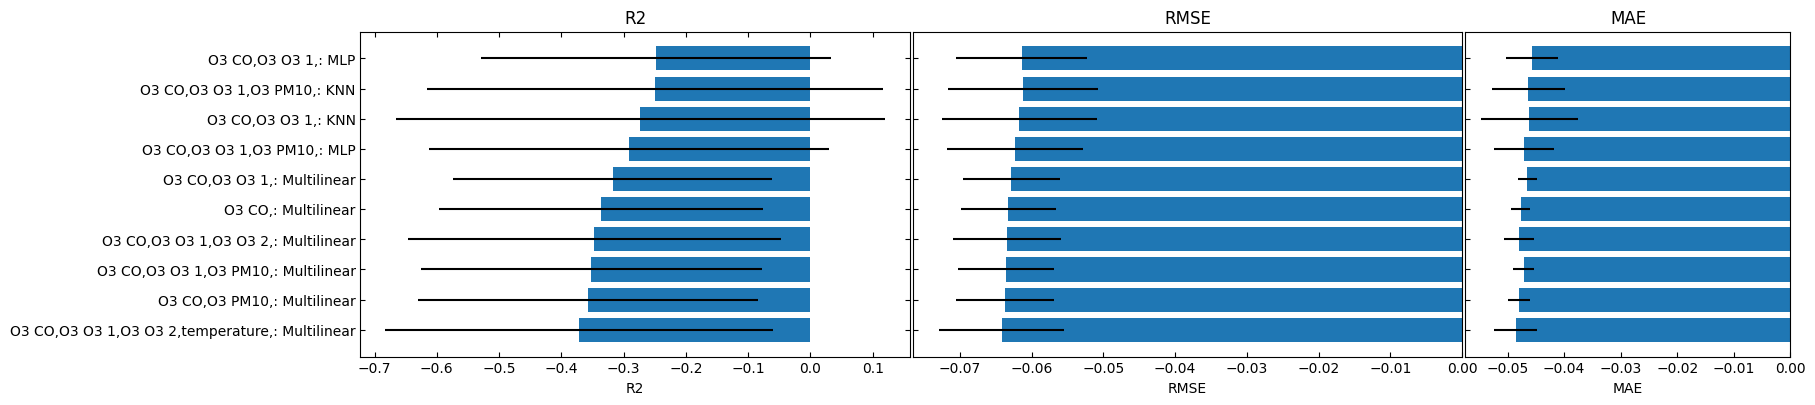
\includegraphics[width=\textwidth]{chapters/3-ANÁLISE DOS DADOS/Figuras/co-all-models-performance.png}
    \label{fig:data-co-all-models-performance}
    \fonte{Desenvolvido pelo autor (2023)}
\end{figure}

A Figura \ref{fig:data-co-all-models-comparison} mostra uma comparação do desempenho, em termos do valor médio de R2, de cada modelo de regressão aplicado para diferentes combinações de variáveis de entrada.

\begin{figure}[h]
    \centering
    \caption{Comparação dos modelos de calibração aplicados as leituras de \acrshort{co} do sensor CO-B4}
    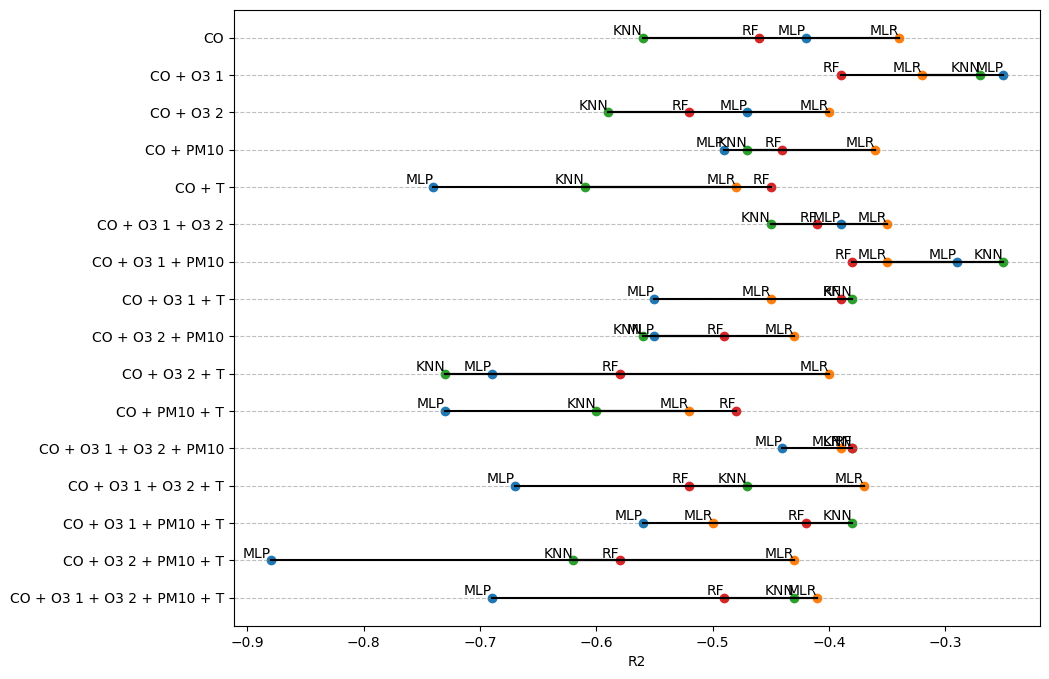
\includegraphics[width=\textwidth]{chapters/3-ANÁLISE DOS DADOS/Figuras/co-all-models-comparison.png}
    \label{fig:data-co-all-models-comparison}
    \fonte{Desenvolvido pelo autor (2023)}
\end{figure}

\subsubsection{Calibração das leituras de \acrshort{o3}}

A Figura \ref{fig:data-o3-all-models-performance} apresenta os valores de R2 dos 10 melhores modelos de calibração calculados para as leituras de \acrshort{o3}. Observa-se que apesar do valor médio de R2 obtido nas validações cruzadas continuar sendo negativo, obtiveram-se máximos de aproximadamente 0.1 para alguns conjuntos de dados ao utilizar regressões com k vizinhos mais próximos considerando as leituras de \acrshort{co} e \acrshort{mp10}.

\begin{figure}[h]
    \centering
    \caption{Resultados dos 10 melhores modelos de calibração aplicados as leituras de \acrshort{o3} do sensor OX-B431}
    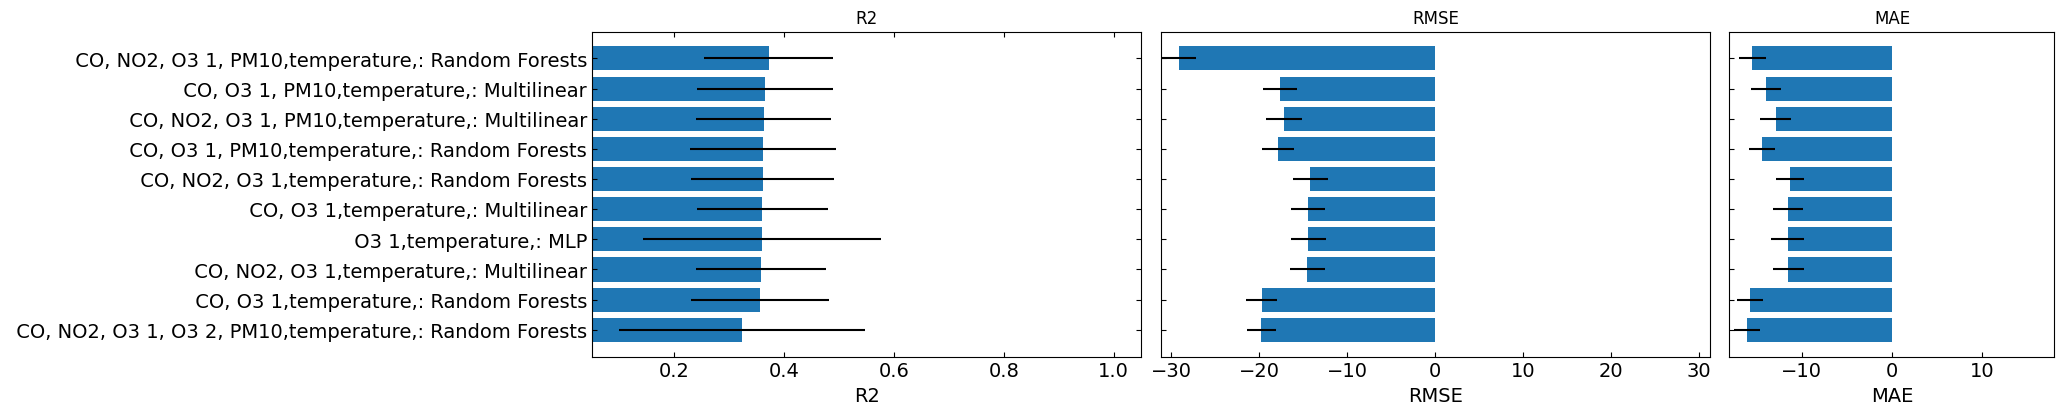
\includegraphics[width=\textwidth]{chapters/3-ANÁLISE DOS DADOS/Figuras/o3-all-models-performance.png}
    \label{fig:data-o3-all-models-performance}
    \fonte{Desenvolvido pelo autor (2023)}
\end{figure}

A Figura \ref{fig:data-o3-all-models-comparison} mostra uma comparação do desempenho, em termos do valor médio de R2, de cada modelo de regressão aplicado para diferentes combinações de variáveis de entrada.

\begin{figure}[h]
    \centering
    \caption{Comparação dos modelos de calibração aplicados as leituras de \acrshort{o3} do sensor OX-B431}
    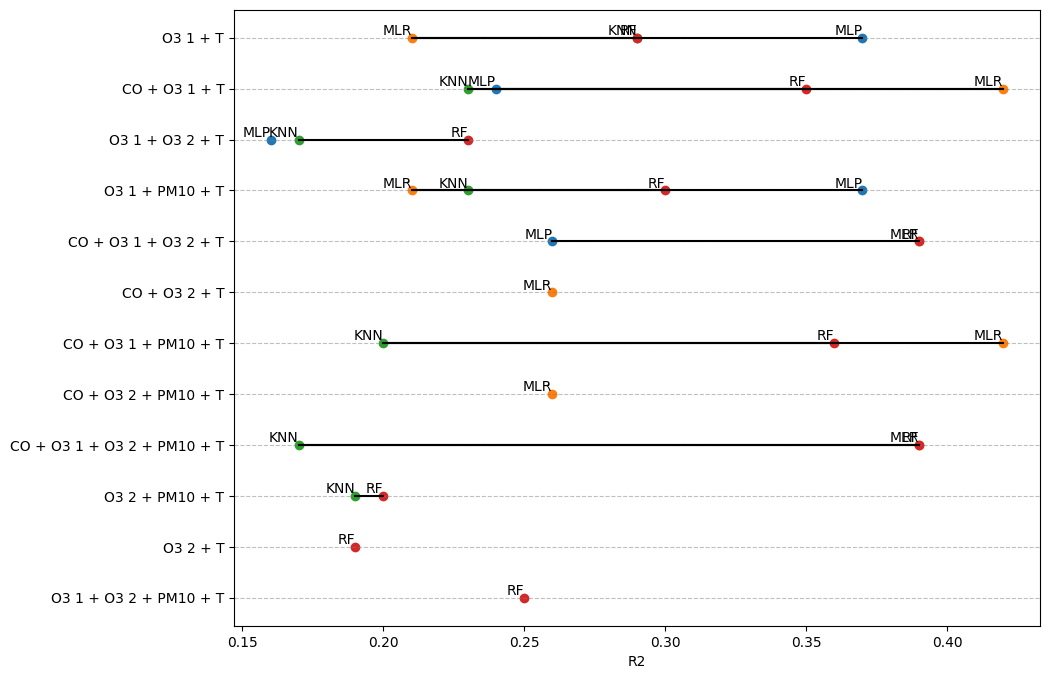
\includegraphics[width=\textwidth]{chapters/3-ANÁLISE DOS DADOS/Figuras/o3-all-models-comparison.png}
    \label{fig:data-o3-all-models-comparison}
    \fonte{Desenvolvido pelo autor (2023)}
\end{figure}

\subsubsection{Calibração das leituras de \acrshort{mp10}}

A Figura \ref{fig:data-pm10-all-models-performance} apresenta os valores de R2 dos 10 melhores modelos de calibração calculados para as leituras de \acrshort{mp10}. Observa-se que apesar do valor médio de R2 obtido nas validações cruzadas continuar sendo negativo, obtiveram-se máximos de aproximadamente 0.1 para alguns conjuntos de dados ao utilizar regressões com k vizinhos mais próximos considerando as leituras de \acrshort{o3} e \acrshort{mp10}.

\begin{figure}[h]
    \centering
    \caption{Resultados dos 10 melhores modelos de calibração aplicados as leituras de \acrshort{mp10} do sensor OPC-N3}
    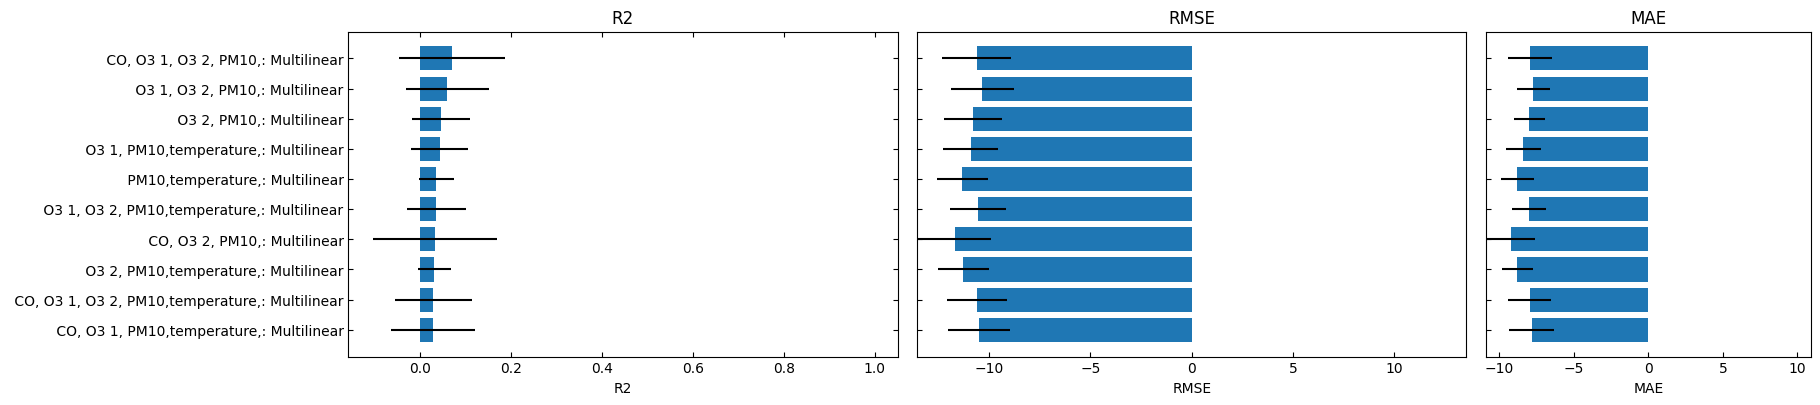
\includegraphics[width=\textwidth]{chapters/3-ANÁLISE DOS DADOS/Figuras/pm10-all-models-performance.png}
    \label{fig:data-pm10-all-models-performance}
    \fonte{Desenvolvido pelo autor (2023)}
\end{figure}

A Figura \ref{fig:data-pm10-all-models-comparison} mostra uma comparação do desempenho, em termos do valor médio de R2, de cada modelo de regressão aplicado para diferentes combinações de variáveis de entrada.

\begin{figure}[h]
    \centering
    \caption{Comparação dos modelos de calibração aplicados as leituras de \acrshort{mp10} do sensor OPC-N3}
    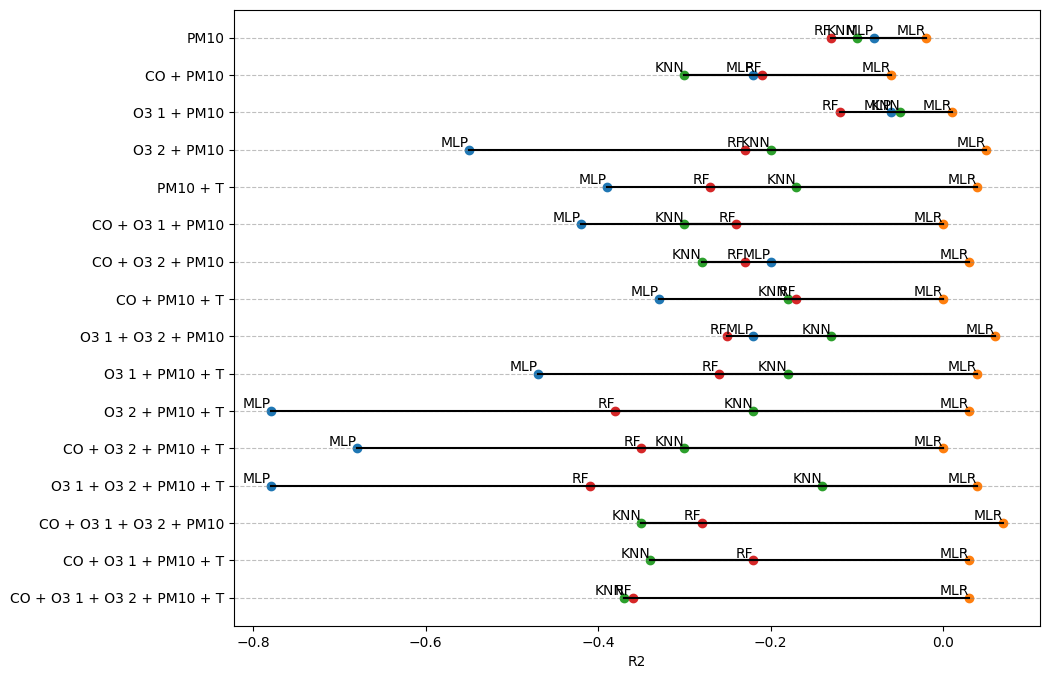
\includegraphics[width=\textwidth]{chapters/3-ANÁLISE DOS DADOS/Figuras/pm10-all-models-comparison.png}
    \label{fig:data-pm10-all-models-comparison}
    \fonte{Desenvolvido pelo autor (2023)}
\end{figure}
